% $Id: template.tex 11 2007-04-03 22:25:53Z jpeltier $

\documentclass{vgtc}                          % final (conference style)
%\documentclass[review]{vgtc}                 % review
%\documentclass[widereview]{vgtc}             % wide-spaced review
%\documentclass[preprint]{vgtc}               % preprint
%\documentclass[electronic]{vgtc}             % electronic version

%% Uncomment one of the lines above depending on where your paper is
%% in the conference process. ``review'' and ``widereview'' are for review
%% submission, ``preprint'' is for pre-publication, and the final version
%% doesn't use a specific qualifier. Further, ``electronic'' includes
%% hyperreferences for more convenient online viewing.

%% Please use one of the ``review'' options in combination with the
%% assigned online id (see below) ONLY if your paper uses a double blind
%% review process. Some conferences, like IEEE Vis and InfoVis, have NOT
%% in the past.

%% Figures should be in CMYK or Grey scale format, otherwise, colour 
%% shifting may occur during the printing process.

%% These few lines make a distinction between latex and pdflatex calls and they
%% bring in essential packages for graphics and font handling.
%% Note that due to the \DeclareGraphicsExtensions{} call it is no longer necessary
%% to provide the the path and extension of a graphics file:
%% \includegraphics{diamondrule} is completely sufficient.
%%
\ifpdf%                                % if we use pdflatex
  \pdfoutput=1\relax                   % create PDFs from pdfLaTeX
  \pdfcompresslevel=9                  % PDF Compression
  \pdfoptionpdfminorversion=7          % create PDF 1.7
  \ExecuteOptions{pdftex}
  \usepackage{graphicx}                % allow us to embed graphics files
  \DeclareGraphicsExtensions{.pdf,.png,.jpg,.jpeg} % for pdflatex we expect .pdf, .png, or .jpg files
\else%                                 % else we use pure latex
  \ExecuteOptions{dvips}
  \usepackage{graphicx}                % allow us to embed graphics files
  \DeclareGraphicsExtensions{.eps}     % for pure latex we expect eps files
\fi%

%% it is recomended to use ``\autoref{sec:bla}'' instead of ``Fig.~\ref{sec:bla}''
\graphicspath{{figures/}{pictures/}{images/}{./}} % where to search for the images

\usepackage{microtype}                 % use micro-typography (slightly more compact, better to read)
\PassOptionsToPackage{warn}{textcomp}  % to address font issues with \textrightarrow
\usepackage{textcomp}                  % use better special symbols
\usepackage{mathptmx}                  % use matching math font
\usepackage{times}                     % we use Times as the main font
\renewcommand*\ttdefault{txtt}         % a nicer typewriter font
\usepackage{cite}                      % needed to automatically sort the references
\usepackage{tabu}                      % only used for the table example
\usepackage{booktabs}                  % only used for the table example
\usepackage{enumitem}
\usepackage{xspace}
\usepackage[percent]{overpic}
\usepackage{tikz}
% \usepackage{svg}
\usepackage{amsmath}
%\usepackage{xcolor}
%\usepackage[dvipsnames]{xcolor}
\usepackage{array}
\usepackage[export]{adjustbox}
\usepackage{graphbox}
\usepackage{tabularx}
\usepackage{float}
\usepackage{transparent}

%% We encourage the use of mathptmx for consistent usage of times font
%% throughout the proceedings. However, if you encounter conflicts
%% with other math-related packages, you may want to disable it.




\newcommand{\jdf}[1]{\textcolor{blue}{jdf: #1}}
\newcommand*\circled[1]{\tikz[baseline=(char.base)]{
            \node[shape=circle,draw,inner sep=2pt] (char) {#1};}}
\newcommand*\circledColored[2]{\tikz[baseline=(char.base)]{
            \node[#2,shape=circle,draw,inner sep=2pt] (char) {#1};}}
\newcommand{\ts}{\textsuperscript}

\newcommand{\model}{bipartite multivariate dynamic network\xspace}
\newcommand{\modelplural}{bipartite multivariate dynamic networks\xspace}

%% If you are submitting a paper to a conference for review with a double
%% blind reviewing process, please replace the value ``0'' below with your
%% OnlineID. Otherwise, you may safely leave it at ``0''.
\onlineid{0}

%% declare the category of your paper, only shown in review mode
\vgtccategory{Research}

%% allow for this line if you want the electronic option to work properly
\vgtcinsertpkg

%% In preprint mode you may define your own headline.
%\preprinttext{To appear in an IEEE VGTC sponsored conference.}

%% Paper title.

\title{From Historical Documents To Social Network Visualization: Potential Pitfalls and Network Modeling}

%% This is how authors are specified in the conference style

%% Author and Affiliation (single author).
%%\author{Roy G. Biv\thanks{e-mail: roy.g.biv@aol.com}}
%%\affiliation{\scriptsize Allied Widgets Research}

%% Author and Affiliation (multiple authors with single affiliations).
%%\author{Roy G. Biv\thanks{e-mail: roy.g.biv@aol.com} %
%%\and Ed Grimley\thanks{e-mail:ed.grimley@aol.com} %
%%\and Martha Stewart\thanks{e-mail:martha.stewart@marthastewart.com}}
%%\affiliation{\scriptsize Martha Stewart Enterprises \\ Microsoft Research}

%% Author and Affiliation (multiple authors with multiple affiliations)
% \author{Roy G. Biv\thanks{e-mail: roy.g.biv@aol.com}\\ %
%         \scriptsize Starbucks Research %
% \and Ed Grimley\thanks{e-mail: ed.grimley@aol.com}\\ %
%      \scriptsize Grimley Widgets, Inc. %
% \and Martha Stewart\thanks{e-mail: martha.stewart@marthastewart.com}\\ %
%      \parbox{1.4in}{\scriptsize \centering Martha Stewart Enterprises \\ Microsoft Research}}

%% A teaser figure can be included as follows, but is not recommended since
%% the space is now taken up by a full width abstract.
%\teaser{
%  \includegraphics[width=1.5in]{sample.eps}
%  \caption{Lookit! Lookit!}
%}

%% Abstract section.
\abstract{
    Historical Social Network Analysis (HSNA) is a branch of history where historians model and study sociological phenomena of the past through the lens of networks. For that, they retrieve information about the social relationships of a period and place they study from historical documents, that they model using a network. However, the process of constructing a network from historical sources is not trivial and can lead to distortion and traceability problems. In this paper, we discuss the different steps of an HSNA workflow, along the potential drawbacks of each steps which can result in bias in the final analysis. We discuss in depths the network modeling step and argue that the first constructed network in an analysis should satisfy reality and traceability properties in regard of the original documents. We discuss the bipartite dynamic multivariate network model which satisfy these properties and can be used to model well the majority of historical documents we encountered. 
%
} % end of abstract

%% ACM Computing Classification System (CCS). 
%% See <http://www.acm.org/about/class> for details.
%% We recommend the 2012 system <http://www.acm.org/about/class/class/2012>
%% For the 2012 system use the ``\CCScatTwelve'' which command takes four arguments.
%% The 1998 system <http://www.acm.org/about/class/class/2012> is still possible
%% For the 1998 system use the ``\CCScat'' which command takes four arguments.
%% In both cases the last two arguments (1998) or last three (2012) can be empty.

\CCScatlist{
  \CCScatTwelve{Human-centered computing}{Visu\-al\-iza\-tion}{Visu\-al\-iza\-tion techniques}{Treemaps};
  \CCScatTwelve{Human-centered computing}{Visu\-al\-iza\-tion}{Visualization design and evaluation methods}{}
}

%\CCScatlist{
  %\CCScat{H.5.2}{User Interfaces}{User Interfaces}{Graphical user interfaces (GUI)}{};
  %\CCScat{H.5.m}{Information Interfaces and Presentation}{Miscellaneous}{}{}
%}

%% Copyright space is enabled by default as required by guidelines.
%% It is disabled by the 'review' option or via the following command:
% \nocopyrightspace

%%%%%%%%%%%%%%%%%%%%%%%%%%%%%%%%%%%%%%%%%%%%%%%%%%%%%%%%%%%%%%%%
%%%%%%%%%%%%%%%%%%%%%% START OF THE PAPER %%%%%%%%%%%%%%%%%%%%%%
%%%%%%%%%%%%%%%%%%%%%%%%%%%%%%%%%%%%%%%%%%%%%%%%%%%%%%%%%%%%%%%%%

\begin{document}

%% The ``\maketitle'' command must be the first command after the
%% ``\begin{document}'' command. It prepares and prints the title block.

%% the only exception to this rule is the \firstsection command
\firstsection{Introduction}

\maketitle

% Social historians' goal is to characterize socio-economic phenomena and their dynamics on a restricted period and place of interest, and see how individual people of that time lived through them. For this, they rely on historical documents such as conversational letters, census, marriage acts etc. They usually extract qualitative and quantitative information from an identified corpus of documents, to then make quantitative conclusions on interesting socio-economic patterns. This can range from the distribution of jobs and social status, the migratory flux, to the structure of families in a given society. For this, historians can follow a Social Network Analysis (SNA) or more precisely a Historical Social Network Analysis (HSNA) approach. HSNA is a method---sometimes referred as a paradigm---which consists in modeling the social relationships between a set of entities---usually individuals---into a network, using the information from the historical documents. Very often, historians model the persons mentioned in the text as the nodes of the network, who are connected two by two by links modeling social relationships, such as friendships and family ties.
% However, textual sources can be rich in information and can refer to complex relationships involving more than two persons at the same time. Persons can also have different implications or roles as social relationships are often non symmetrical.
% For example, there have been several studies on business documents concerning financial transactions. These documents often involve more than two persons, who can have very different roles. Usually this type of document refers to sellers and buyers, but can also indicate other persons such as a guarantor, and/or some kind of notary. These complex relationships are hard to model into simple person-to-person networks.
% Furthermore, textual sources almost always contain extra information in regard of the event they refer to like the time, location, and other such as the type and amount of the transaction. It can also contain extra information about the persons such as their job, family and sex.
% It is clear that such information-rich data is difficult to model as person-to-person simple network. Even if more complex models have been proposed in the literature, such as dynamic or bipartite networks, simple networks are still the norm. In this paper, we first describe the social historians work process when they follow an HSNA, starting from the textual sources acquisition to the analysis and visualization of the network, and we identify potential fallback at each steps.
% Then, after describing the most used network models in HSNA, we formalize a network model which models well the majority of historical sources we encountered in all their complexity: \model. We give real world example on how this model has been used to follow HSNA pipelines, from data preparation to visual analysis using a visual query system. From these examples, we identify 3 properties of this model compared to simple networks: non-duplication of information, no ambiguity, and concordance of the original sources.


Social historians' goal is to characterize socio-economic phenomena and their dynamics on a restricted period and place of interest, and see how individual people of that time lived through them. For this, they rely on historical documents such as conversational letters, census, marriage acts etc. They usually extract qualitative and quantitative information from an identified corpus of documents, to then make quantitative conclusions on interesting socio-economic patterns. This can range from the distribution of jobs and social status, the migratory flux, to the structure of families in a given society. For this, historians can follow a Social Network Analysis (SNA) or more precisely a Historical Social Network Analysis (HSNA) approach. HSNA is a method---sometimes referred as a paradigm---which consists in modeling the social relationships between a set of entities---usually individuals---into a network, using the textual information of the historical documents.
Very often, historians model the persons mentioned in the text as the nodes of the network, who are connected two by two by links modeling social relationships, such as friendships and family ties.
However, historical documents are often rich in information and can refer to complex relationships involving more than two persons at the same time. Persons can also have different implications or roles in the documents are relationships are often non symmetrical \cite{lemercier_analyse_2005}.
For example, there have been several studies on business documents concerning financial transactions. These documents often involve more than two persons, who can have very different roles. Usually this type of document refers to sellers and buyers, but can also indicate other persons such as a guarantor, and/or some kind of notary. These complex relationships are hard to model into simple person-to-person networks.
Furthermore, textual sources almost always contain extra information in regard of the event they refer to like the time, location, and other such as the type and amount of the transaction. It can also contain extra information about the persons such as their job, family and sex.
It is clear that such information-rich data is difficult to model as person-to-person simple network. Even if more complex models have been proposed in the literature, such as dynamic or bipartite networks, simple networks are still the norm.
Moreover, lots of HSNA studies focus on reporting network analysis results, but rarely give details on the annotation and network modeling process, which is yet primordial as it influence greatly the final network shape. Therefore, it can be difficult for readers to trace back the analysis to the original documents, and can pose replicability problems \cite{baker_1500_2016}. For these reasons, network models which can represent the complex reality of the documents and allow a traceability to the sources are needed.  
In this paper, we first describe the social historians work process when they follow an HSNA, starting from the textual sources acquisition to the analysis and visualization of the network, and we identify potential drawbacks for each step.
Then, after describing the most used network models in HSNA, we formalize a network model which satisfy \textit{reality} and \textit{traceability} properties, and
which models well the majority of historical sources we encountered in all their complexity: the \model. We give real world examples on how this model has been used to follow HSNA pipelines, from data preparation to visual analysis using a visual query system. From these examples, we identify 3 properties of this model compared to simple networks: non-duplication of information, no ambiguity, and concordance to the original sources.

\section{Related Work}

\subsection{Social Network Analysis}

In Sociology networks always have been a common metaphor to talk about the social ties inside a group, which form a web of different relations. After a lot of work in graph theory and network modeling in the 1950s, sociologists started to appropriate those concepts to themselves and use them to model social relations---such as family, friendships or business ties---with networks. SNA revolutionised classical Sociology by trying to explain social phenomena through the lens of real interactions modeled as networks, while classical methods were revolving around predefined social groups such as the age, job, sex and social status. 
History started to use those concepts in the 1980s, to study individuals and groups through the lens of their interactions and relationships directly extracted from historical documents. It followed social history which was already revolving about extracting quantitative information from documents in an exhaustive way, to to make socio-economic conclusions on a period of interest. Since then, HSNA has been applied to study various things, from family structures to maritime business.

\subsection{Network Modeling}

Social scientists started to model social relationships using a simple graph $G= (V, E)$ with V a set a vertices representing actors---very often persons---and $E \subseteq V^2$ a set of edges modeling the social ties between pairs of actors \cite{freeman_development_2004}.

The (H)SNA network models have evolved in time to better take into account real properties of social networks, such as types of actors using labeled networks, importance of actors or relations with weighted networks, dynamics of relations with dynamic networks.
Bipartite networks have been proposed to model relations between two types of entities, such as organization and employees where the relations link employees to organizations but not employees to employees or organizations to organizations.
Multivariate networks, i.e.,  graphs where vertices and edges can be assigned multiple ``properties'' or ``attributes'' are less used in SNA\@. These attributes are often considered secondary, the emphasis of SNA being on the graph topology, its features, measures, and evolution.

Historians, demographers, sociologists, and anthropologists have been designing specific data models for their social networks, based on genealogy or more generally kinship~\cite{hamberger:halshs-00658667}. For genealogy, the standard GEDCOM~\cite{gedcom} format models a genealogical graph as a bipartite graph with two types of vertices: individuals and families. The PUCK software~\cite{PUCK} has extended the GEDCOM format to adapt to more flexible kinds of family structures for anthropology studies.

\subsection{Social Network Visualization}

Social scientists such as sociologists and historians always used visual representations to gain a better understanding of networks they were studying. Moreno elaborated sociograms in the 1930s to visually represent friendships in a node-link fashion \cite{moreno_foundations_1941}. Node-link diagrams are still the most used technique in SNA and HSNA by far to represent networks, even though its lack of readability for medium to large networks. The most used social network visual analytics softwares such as Gephi \cite{Gephi} and Pajek \cite{batagelj_pajek_nodate} are based on this type of representations and allow a fully integrated exploration and analysis with the help of various algorithms.
The visualization community also proposed other representations to visualize and explore other types of networks such as PAOHVis \cite{valdivia_analyzing_2021} for dynamic hypergraphs and NodeTrix for clustered graphs \cite{henry2007nodetrix}.
Lots of of Visual Analytics tools have been proposed to explore and analyze social networks, often combining several coordinated representations to allow an analysis according various dimensions, such as Jigsaw \cite{Stasko} and the Vistorian \cite{bach_networkcube_nodate}. 


\section{Historians workflow}

When following an HSNA, historians' goals is to characterize structural and individual patterns of sociability between actors of a given period and place. For this, they construct a network modeling social ties between actors using their sources, and analyze and visualize it to make high level social conclusions. This process is not straightforward and can be split into five steps, based on the literature \cite{dufournaud_recherche_2015} and discussions we had with social historians on their work process: \textit{textual sources acquisition}, \textit{numerization}, \textit{annotation}, \textit{network construction} and finally \textit{visualization} and \textit{analysis}.

\subsection{Textual Sources Acquisition}

Historians' first step is to gather a set of textual documents mentioning people who will have social ties between them. For this, they usually take documents from a specific source---such as a national archive---and restrict to a period and place. They also often restrict themselves to one document type, for example marriage acts, to restrict the analysis to one or few types of social ties and to ease the process. Once they restricted their search to documents type, time and place, they want to exhaustively find all the documents satisfying these constraints, as missing documents result in uncertainty in the resulting network and thus the conclusions.

\subsection{Numerization}

Numerization is the only accessory step of the process, as everything can in theory be done without a computer, as it was the case in the past when historians where working mostly in the archive rooms with paper and pens. However, numerization is now always done as it allows to tremendously ease the storage, indexation and annotations of the documents, and facilitate the creation of a network object afterwards.
Numerization can be done by hand or with the help of Optical Character Recognition (OCR) tools. However, if OCR tools are more and more efficient in English and highly used languages, historians work with old documents written in old or extinguished languages, and with atypical written style. Therefor, OCR tools are rarely used.  

\subsection{Annotation}

Annotation is the process of finding and extracting useful information from the documents, concerning the persons, their social ties and any useful information for the historian. These extra information can concern the persons (their age, profession, sex, ethnicity etc) and their social relationships (type, date, place).
Historians also sometimes annotate information on other entities mentioned in the documents, such as art objects or administrative entities. 
Usually, historians have a first idea of what they want to annotate in the data as they already explored the documents and have knowledge on their subject of study, with hypotheses they want to explore. It is however common they can change their mind through the annotation process, by reflecting on what they found in the documents. 
This task is not trivial and the choice of annotations will have an impact on the final network. Historians often have an idea of the network they want to build before the annotation process. 
The Text Encoding Initiative (TEI)~\cite{TEI} is an XML vocabulary and a set of guidelines typically used to encode and annotate documents, and the events happening in these documents (unclear parts, gaps, mistakes, etc.). It is also used for historical texts and to generate social networks~\cite{dufournaud_comparaison_2006}.
% Several softwares can be used for annotation and are usually stored in markups formats such as XML .

\subsection{Network Transformation}

Historians construct a network from the annotations of the documents. Usually, all persons mentioned are annotated and will be transformed into nodes. Additional information such as their age, profession and gender can be stored as node attributes. 
How the network's links are created is not as trivial and can vary a lot. The most straightforward approach is to create a link between every pair of persons mentioned in one document, thus forming a clique motif. This is a simplistic heuristic as persons very often have different roles in the documents.
A more factual approach consists in differentiating the roles of the persons in the documents and modeling them as link types. For example, for marriage acts, the witnesses will be linked with the spouses with a \textit{witness} link, while the spouses will be linked together with a \textit{spouse} link. However, there are often several possible representations, as the social relationships include several people and are difficult to represent as pairwise ties. For example, witnesses can be linked to one, or both of the spouses depending on the analysis goals. If a priest is leading the ceremony, he could be linked to the spouses, or the spouses and the witnesses.
Furthermore, for both examples, there is a loss of information concerning the precise events and we may not retrieve who was mentioned in the exact same documents from the network alone. For example, if someone marry twice, we may not know which marriage the witnesses are from.
To counter these issues, some historians transform their sources into bipartite networks (also called 2-modes and affiliation networks), where the sources are also modeled as nodes and the links model the occurrences of a person in a document, with their roles.

\subsection{Network Analysis and Visualization}

Once historians constructed a network they are satisfied with, they start exploring and analyzing it with visualization and quantitative methods. 
There is traditionally two schools of thought in SNA : Structuralism and Ego studies \cite{eve_deux_2002}. Structuralists are interested in studying the structure and properties of the network, and leverage those to make conclusions on real social phenomena. 
In contrary, sociologists using ego networks focused more on specific individuals, and tried to model all their social interactions whatever the type to understand other sociological attributes such as their status, or certain behaviours. This school is thus often using ego networks, multiplex relationships and dynamic networks.
Most HSNA studies usually involve concepts and methods from these two approaches, trying to make structural conclusions on how an organization operates while observing specific individuals in their complexity.
During the analysis, historians use visualization tools to gain a better understanding of the network's structure. It allows them to explore the network and detect interesting patterns rapidly. Most widely used tools are Pajek and Gephi, which also provide algorithms for the analysis, such as for community detection or structural analysis.


\begin{figure}[tb]
 \centering % avoid the use of \begin{center}...\end{center} and use \centering instead (more compact)
 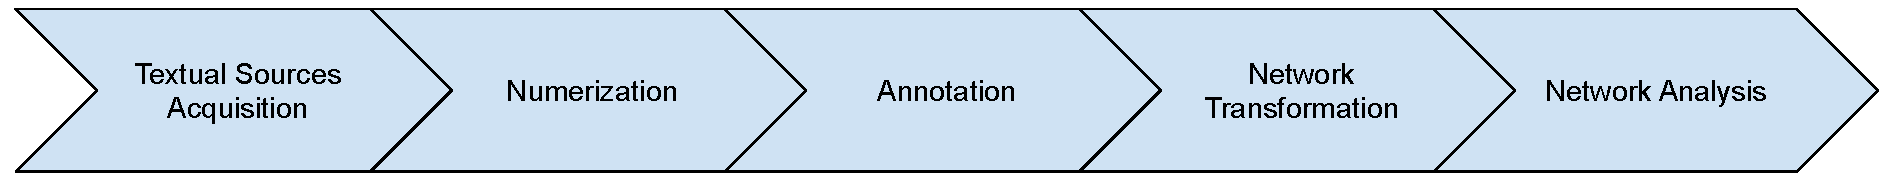
\includegraphics[width=\columnwidth]{Figures/process.pdf}
 \caption{HSNA process}
 \label{fig:sample}
\end{figure}




% \begin{table}[h]
% \begin{tabularx}{\textwidth}{|l|X|}

\begin{table}[h]
\begin{tabularx}{\columnwidth}{|p{2cm}|X|}
\hline
Textual Sources Acquisition & F1. Too many missing documents (data not exhaustive)  \\ \hline
Numerization                & F2: Wrong character recognition \\ \hline
Annotation                         & F3: Missing annotations \newline F4: Non systematic annotation schema              \\ \hline
Network Creation                   & F5: Wrong duplication and merging of entities\newline F6: Bad network model choice \\ \hline
Network Visualization and Analysis & F7: Bad choice of visualizations\newline F8: Bad choice of algorithms/measures                 \\ \hline
\end{tabularx}
\end{table}

% \begin{table}[]
% \begin{tabular}{|l|l|}
% \hline
% Textual Sources Acquisition & F1. Too many missing documents  \\ \hline
% Numerization                & F2: Wrong character recognition \\ \hline
% Annotation                         & \begin{tabular}[c]{@{}l@{}}F3: Missing annotations\\ F4: Non systematic annotation schema\end{tabular}               \\ \hline
% Network Creation                   & \begin{tabular}[c]{@{}l@{}}F5: Wrong duplication and merging of entities\\ F6: Bad network model choice\end{tabular} \\ \hline
% Network Visualization and Analysis & \begin{tabular}[c]{@{}l@{}}F7: Bad choice of visualizations\\ F8: Bad choice of metrics\end{tabular}                 \\ \hline
% \end{tabular}
% \end{table}


\section{Network modeling and analysis}

\subsection{History and Computer Science}

Traditionally, historians try to tell a story about protagonists and socio-economic facts in a given society. This narrative approach of history have been criticized for its lack of traceability and the open interpretation of historical documents, which can introduce bias of the author.
Social history and HSNA were a response to this problem, by bringing quantitative methods to enforce a narrative supported by data and statistical results. However, traditional HSNA studies describe globally their sources without precising the annotation and transformation process they followed. They don't mention how the network they study has been obtained from the sources. Yet, these steps are critical as they can deeply influence the results of the analysis \cite{cristofoli_aux_2008}. Indeed, historians have to make choices on what to annotate and what to model into the network. This often depends on what they want to demonstrate at the end.
As these steps of the workflow are often not transparent, it can be difficult for the reader of an HSNA study to understand how does the network has been constructed, what it represents, and to trace back the network entities from the original sources \cite{dufournaud_recherche_2015}. 

Recently, Experimental Computer Science went through a replicability crisis, pointing out that a lot of results were not reproducible, since authors were not giving enough data or information for people to redo the same analysis \cite{baker_1500_2016}. Reproducibility is though considered a condition for building scientific knowledge, and this discussion highlighted the fragility of a lot of experimental studies. Data shows that the natural and social sciences are also affected.

Usage of computer science in history can mitigate this problem, by providing methods and tools for historians to follow their analysis and providing traceability from their high level conclusions to the original documents. 

We think one way of doing that is to use a network model which reflects well the \textbf{reality} of the social relationships mentioned in the documents, and are \textbf{traceable} to the original sources. We think network models which satisfy these two properties---\textbf{reality} and \textbf{traceability}---should always be constructed from the original sources as a basis for the analysis. Other network transformations can be applied afterwards to reveal specific patterns, but having a network which reflects well the reality of the documents is primordial for representing the sources as they are, and allowing to easily go back from them at any point in the analysis. Indeed, any transformation can be applied from a network representing well the sources. But applying modifications and transformations directly in the annotation process can bias the analysis and remove the possibilities to follow other explorations and hypothesis in the future.

\subsection{Network Models}

Currently, historians use various network models depending of their knowledge of network science, the structure of their sources and annotations, and the analysis they plan to make. We describe here the most used network models in the HSNA literature:

% Once historians have annotated their corpus with the persons, their social relationships, and any other information related to the persons and the documents---such as the time and location---they have several ways of constructing a network [REF PASCAL]. We describe here the most used network models from the HNR literature:
\begin{itemize}[noitemsep]
    \item \textbf{Co-occurrence Network:} Only the persons are represented as nodes, and two persons are connected with a link when they are mentioned in the same document. This is the most simple model and was the first to have been used in SNA and HSNA. The major drawback of this model is that it does not take into account the diversity of social relationships, as every link is similar. It can work well when only one type of social relationship is studied like a friendship network [REF schoolers]. However, historical documents rarely mention only one type of relationship. Therefore this model is very limiting for HSNA.
    \item \textbf{Multiplex unipartite network:} Only the persons are represented as nodes, and links model social ties between two persons. Links can have different types, which each represents a different type of social relationships. It allows to model more complex social dynamics where people can have various social ties, such as parent, family and working relationships. One of the main drawback of this model is that very often several coexistent possible representations for the same data exist, especially for complex relationships.
    \item \textbf{Bipartite (also called 2-mode and affiliation) Networks:} Both the persons and the documents are represented as nodes in this network model. A link refer to a mention of a person in a document, and can thus only occur between persons and documents nodes. Usually links are not typed and only encode occurrences, but more recent analysis in HSNA encoded the role of the persons in the document as link type. This network model allows to have a network model more aligned with the original sources and to follow an analysis through the documents themselves. 
\end{itemize}

In the literature, Unipartite (co-occurence and multiplex) networks are still the norm. However, we believe that if this type of model can be useful for SNA, they often bring distortion and ambiguity for historical datasets, which are often quite complex. Cristofoli argues that using a bipartite network allows to model the social reality with a better alignment with the original sources, and point to the drawbacks of using unipartite projections \cite{cristofoli_aux_2008}.

Moreover, historical sources very often contain extra information related to the persons and events mentioned. For example, it is not rare that a marriage act or a business contract mention the jobs and the ethnicity of the people mentioned. These types of documents also always point the date and location of the event, and sometimes more.
Traditionally, social scientists were not directly modeling this extra information into the network, which was considered as a purely structural object. However, more modern studies try to incorporate this rich information directly in the network with more complex models such as dynamic and multivariate graphs. A lot of work has also been done in visual analytics to explore and analyze these more complex networks.

\subsection{Examples}\label{sec:examples}

We discussed with four historians collaborators at different steps of their HNSA workflow about their work process. Specifically, we discussed about their annotation process and how they wanted to model their network. They all work on semi structured historic documents, mentioning complex relationships. We provide more details in the following:

\newcommand{\pascal}{\#1}
\newcommand{\nicole}{\#2}
\newcommand{\zacarias}{\#3}
\newcommand{\dana}{\#4}
\newcommand{\myindent}{~~} % ~\rule{1pt}{6pt}
\begin{enumerate}[noitemsep]
    \item Analysis of the social dynamics from \textbf{construction contracts in Italy in the 18\ts{th} century\cite{Cristofoli2018}.} 
    The corpus is made of contracts for different types of constructions in the Piedmont area in Italy. People are mentioned in three different roles: \textit{Associates} (S) who participate in the construction, \textit{Guarantors} (G) who bring financial guaranty and \textit{Approvers} (A), who vouch for the guarantors. Documents contain information about the type and materials of constructions, and the origins of people.
    \item Analysis of migrations from the \textbf{genealogy of a french family between the 17\ts{th}--20\ts{th} centuries}.
    The corpus is made of family trees referring to several document/event types: birth and death certificates, marriage acts, military mobilization, and census reports. The roles are different for each event types, and consist in \textit{children, father, mother} for the birth events, \textit{deceased} for the death event, \textit{spouse} and \textit{witnesses} for the marriages, and \textit{family member} for the census events. 
    \item Analysis of migrations from Spain to Argentina through the \textbf{marriage acts at Buenos Aires in the 17--19\ts{th} centuries (1396 acts, 6731 persons)~\cite{moutoukias2016buenos}.}
    The corpus is made of acts that mention the spouses and the witnesses of the wedding, which are the roles modeled by the links. The origin, date of birth and parents names are specified for both spouses.
    % These parenting relationships are important for our collaborator, but do not refer to the same event as the marriage. Thus, we create another event node referencing the birth event, with \textit{father, mother}, \textit{child} as roles and the associated birth year and location as node attributes. 
    \item Socio-political analysis of \textbf{migration of ethnic Germans from communist Romania to West Germany in the 20th century (ongoing work)~\cite{diminescu:hal-02556007}.}
    The corpus is made of administrative forms that mention persons requesting to migrate, along with the persons they want to join, and the administrative persons of the ministry in charge of the forms (3 roles).
    The family members of the aspiring migrant are also mentioned in the forms, with their respective date of birth.
\end{enumerate}

We compare the resulting networks when modeling the data with the three discussed models and when encoding attributes for our 4 collaborations. We do it for one given document. The results are shown in \autoref{tab:models}.
We can clearly see the co-occurence model remove the complexity of the social relationships and only show an abstract "proximity" between individuals.  
Unipartite projections allow to produce meaningful networks which model well the diversity of relations that can link several people. It especially model well simple relationships such as parenting ones as in example \nicole. However, it produces distorsions for more complex relationships involving more than two persons, as in \pascal where people can either be mentioned as associates, guarantors and approbators in the documents. Associates should probably be linked together with \textit{associate} links, but the \textit{guarantors} and \textit{approbators} relationships are more complex to model. Approbators could be linked to the associates, the guarantors or both. The three ways of modeling this type of relation make sense, but can lead to very different network shapes and analysis results. Historians thus have to decide on a transformation among several possibilities, which will probably distort the social reality of the relationships.

Finally, these examples show that when working with multivariate networks, using projections to only have persons as nodes brings problem which is not discussed in the literature which is the duplication of information. Indeed, if a document mentions a date, we can model it as an attribute directly in the document node when using a bipartite model. However, when projecting the network this information appear in the links as many times as there are persons mentioned in the document and often more. For example, if a document mention five people, when creating a co-occurrence Network the time data will appear in the $]\displaystyle\sum_{i=1} ^{4} i = 10$ links created. In contrary, the same information appear only once in a bipartite model.

% \definecolor{temoin}{HTML}{D9EAD3}
% \definecolor{parent}{HTML}{FFF2CC}
% \definecolor{epoux}{HTML}{FCE5CD}
% \definecolor{epouse}{HTML}{D9D2E9}
\definecolor{lightgrey}{gray}{0.9}


\colorlet{temoin}{teal!80!white!50}
\colorlet{parent}{yellow!80!white!50}
\colorlet{epoux}{orange!80!white!50}
\colorlet{epouse}{purple!80!white!50}


\newcommand{\simple}[1][0]{\begin{tikzpicture}[node distance=3cm, auto]
        \node[shape=circle,draw=gray, fill=lightgrey] (A) at (0,1) {A};
        \node[shape=circle,draw=gray, fill=lightgrey] (B) at (2,1) {B};
        \node[shape=circle,draw=gray, fill=lightgrey] (T1) at (1,2) {T1};
        \node[shape=circle,draw=gray, fill=lightgrey] (T2) at (1,0) {T2};
    
        \begin{scope}[every node/.style={scale=.5}]
            \path [line width=0.5mm]
            (A)  edge node [color=black] {\small 1659} (B)
            (T1) edge node [color=black] {\small 1659} (T2)
            (T1) edge node [above left, color=black] {\small 1659} (A)
            (T1) edge node [color=black] {\small 1659} (B)
            (T2) edge node [color=black] {\small 1659} (A)
            (T2) edge node [right, color=black] {\small 1659} (B); 
        \end{scope}
    \end{tikzpicture}}
    

\newcommand{\noParents}[1][0]{\begin{tikzpicture}[->, node distance=3cm, auto]
        \node[shape=circle,draw=gray, fill=lightgrey] (A) at (0,1) {A};
        \node[shape=circle,draw=gray, fill=lightgrey] (B) at (2,1) {B};
        \node[shape=circle,draw=gray, fill=lightgrey] (T1) at (1,2) {T1};
        \node[shape=circle,draw=gray, fill=lightgrey] (T2) at (1,0) {T2};
    
        \begin{scope}[every node/.style={scale=.5}]
            \path [line width=0.5mm] (A) edge [bend left, color=epoux] node [color=black] {\small 1712} (B)
            (B) edge [bend left, color=epouse] node [color=black] {\small 1659} (A)
            (T1) edge [color=temoin] node [above left, color=black] {\small 1659} (A)
            (T1) edge [color=temoin] node [color=black] {\small 1659} (B)
            (T2) edge [color=temoin] node [color=black] {\small 1659} (A)
            (T2) edge [color=temoin] node [right, color=black] {\small 1659} (B); 
        \end{scope}
    \end{tikzpicture}}
    
% \newcommand{\bipartiteNoParents}[1]{\begin{tikzpicture}[, node distance=3cm, auto, scale=#1]
\newcommand{\bipartiteNoParents}[1][0]{\begin{tikzpicture}[, node distance=3cm, auto]
        \node[shape=circle,draw=gray, fill=lightgrey] (A) at (0,3) {H};
        \node[shape=circle,draw=gray, fill=lightgrey] (B) at (0,1) {W};
        
        \node[shape=circle,draw=gray, fill=lightgrey] (T1) at (3,3) {T1};
        \node[shape=circle,draw=gray, fill=lightgrey] (T2) at (3,1) {T2};
        
        \node[shape=rectangle,draw=gray, align=center,fill=lightgrey] (D) at (1.5,2) {M \\[0.5em] \small 1659};
        \draw (D.west) -- (D.east);
    
        \begin{scope}[every node/.style={scale=.5}]
            \path [line width=0.5mm] (A) edge [color=epoux] (D)
            (B) edge [color=epouse] (D)
            (T1) edge [color=temoin] (D)
            (T2) edge [color=temoin] (D);
        \end{scope}
        \end{tikzpicture}}

\newcommand{\unipartiteParents}[1][0]{
\begin{tikzpicture}[->, node distance=3cm, auto]
        \node[shape=circle,draw=gray, fill=lightgrey] (A) at (2,1) {A};
        \node[shape=circle,draw=gray, fill=lightgrey] (B) at (4,1) {B};
        
        \node[shape=circle,draw=gray, fill=lightgrey] (T1) at (3,2) {T1};
        \node[shape=circle,draw=gray, fill=lightgrey] (T2) at (3,0) {T2};
        
        \node[shape=circle,draw=gray, fill=lightgrey] (PA) at (1,2) {PA};
        \node[shape=circle,draw=gray, fill=lightgrey] (MA) at (1,0) {MA};
        
        \node[shape=circle,draw=gray, fill=lightgrey] (PB) at (5,2) {PB};
        \node[shape=circle,draw=gray, fill=lightgrey] (MB) at (5,0) {MB};
    
    \begin{scope}[every node/.style={scale=.5}]
        \path [line width=0.5mm] (A) edge [bend left, color=epoux] node [color=black] {\small 1712} (B)
        (B) edge [bend left, color=epouse] node [color=black] {\small 1712} (A)
        (T1) edge [color=temoin] node [above left, color=black] {\small 1712} (A)
        (T1) edge [color=temoin] node [color=black] {\small 1712} (B)
        (T2) edge [color=temoin] node [color=black] {\small 1712} (A)
        (T2) edge [color=temoin] node [right, color=black] {\small 1712} (B)
        (PA) edge [color=parent] node [color=black] {\small Valencia} (A)
        (MA) edge [color=parent] node [right, color=black] {\small Valencia} (A)
        (PB) edge [color=parent] node [color=black] {\small Valencia} (B)
        (MB) edge [color=parent] node [right, color=black] {\small Valencia} (B);
    \end{scope}
    \end{tikzpicture}
}

\newcommand{\bipartiteParents}[1]{
\begin{tikzpicture}[, node distance=3cm, auto, scale=#1]
        \node[shape=circle,draw=gray, fill=lightgrey] (A) at (0,3) {H};
        \node[shape=circle,draw=gray, fill=lightgrey] (T1) at (0,2) {T1};
        
        \node[shape=circle,draw=gray, fill=lightgrey] (T2) at (0,1) {T2};
        \node[shape=circle,draw=gray, fill=lightgrey] (B) at (0,0) {W};
        
        \node[shape=rectangle,draw=gray, align=center, fill=lightgrey] (D) at (1.5,1.5) {M \\[0.5em] \tiny 1761};
        
        \node[shape=rectangle,draw=gray, align=center, fill=lightgrey] (BA) at (1.5,3) {BA \\[0.5em] \tiny Valencia};
        \node[shape=rectangle,draw=gray, align=center, fill=lightgrey] (BB) at (1.5,0) {BB \\[0.5em] \tiny Valencia};
        
        \draw (D.west) -- (D.east);
        \draw (BA.west) -- (BA.east);
        \draw (BB.west) -- (BB.east);
        
        \node[shape=circle,draw=gray, fill=lightgrey] (PA) at (3,3) {HF};
        \node[shape=circle,draw=gray, fill=lightgrey] (MA) at (3,2) {HM};
        \node[shape=circle,draw=gray, fill=lightgrey] (PB) at (3,1) {WF};
        \node[shape=circle,draw=gray, fill=lightgrey] (MB) at (3,0) {WM};
    
    \begin{scope}[every node/.style={scale=.5}]
        \path [line width=0.5mm] (A) edge [color=epoux] (D)
        (B) edge [color=epouse] (D)
        (T1) edge [color=temoin] (D)
        (T2) edge [color=temoin] (D)
        (PA) edge [color=parent] (BA)
        (MA) edge [color=parent] (BA)
        (PB) edge [color=parent] (BB)
        (MB) edge [color=parent] (BB)
        (A) edge [color=parent] (BA)
        (B) edge [color=parent] (BB);
    \end{scope}
    \end{tikzpicture}
}



\iffalse
\begin{figure}
    \centering
    
%     \begin{subfigure}{0.5\columnwidth}
%     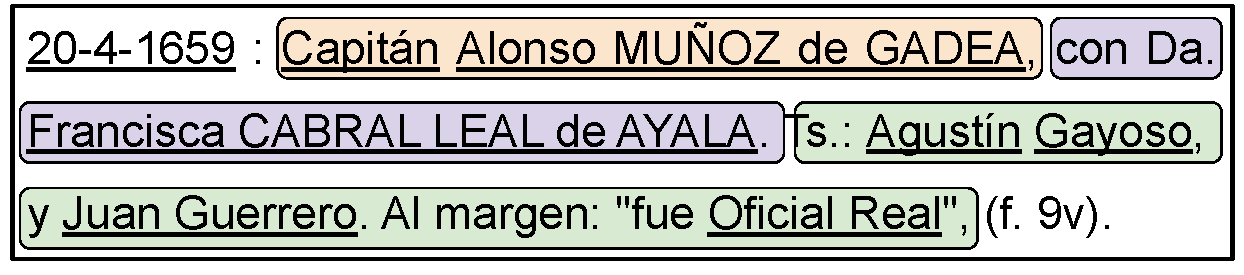
\includegraphics[width=\columnwidth]{Figures/marriageDocumentnoParents.pdf} 
%     % \caption{First, an exciting contribution by unknown artist.}
%   \end{subfigure}
%   \begin{subfigure}{0.32\columnwidth}
%     \bipartiteNoParents{1}
% %   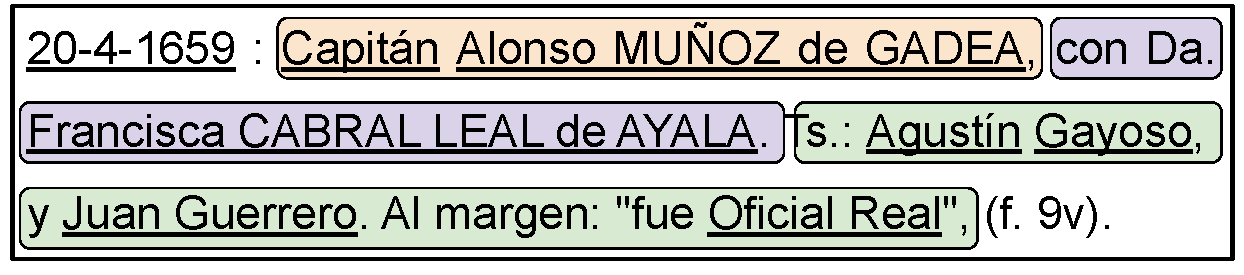
\includegraphics[width=\linewidth]{Figures/marriageDocumentnoParents.pdf} 
% %   \resizebox{0.5\textwidth}{!}{
% %     \bipartiteNoParents{1}
% % }%
%     % \caption{Second, an anonymous mystery.}
%   \end{subfigure}
%   \begin{subfigure}{0.5\columnwidth}
%     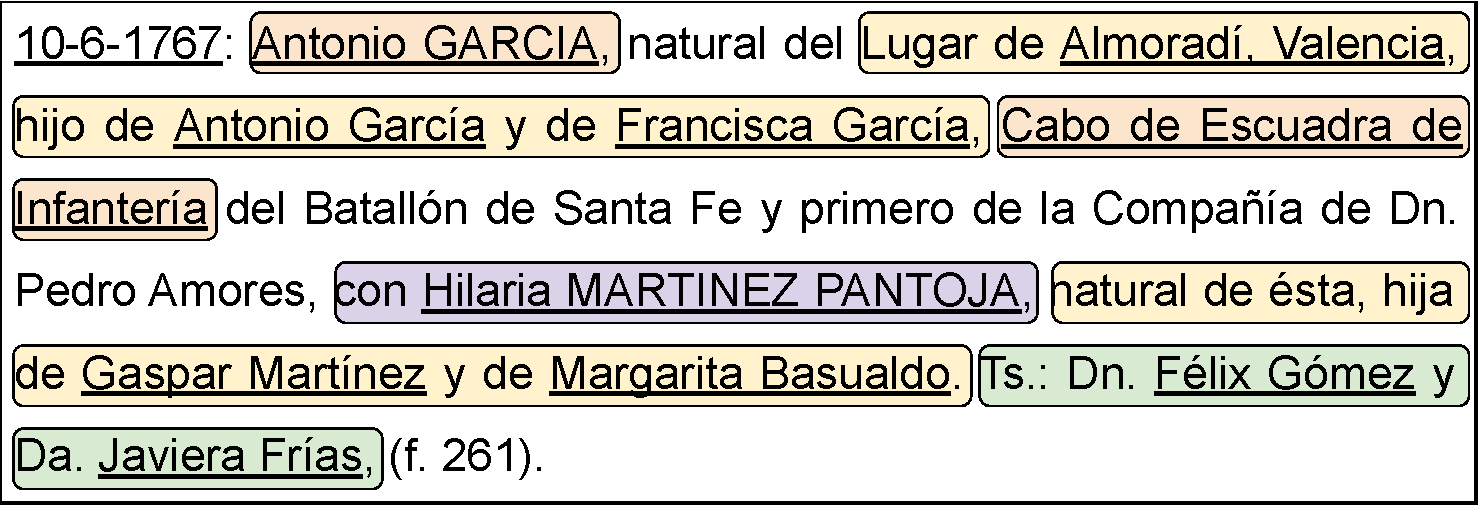
\includegraphics[width=\linewidth]{Figures/marriageDocument.pdf} 
%   \end{subfigure}
%   \begin{subfigure}{0.3\columnwidth}
%     \bipartiteParents{1}
%   \end{subfigure}
  
  
  \begin{subfigure}{.23\textwidth}
    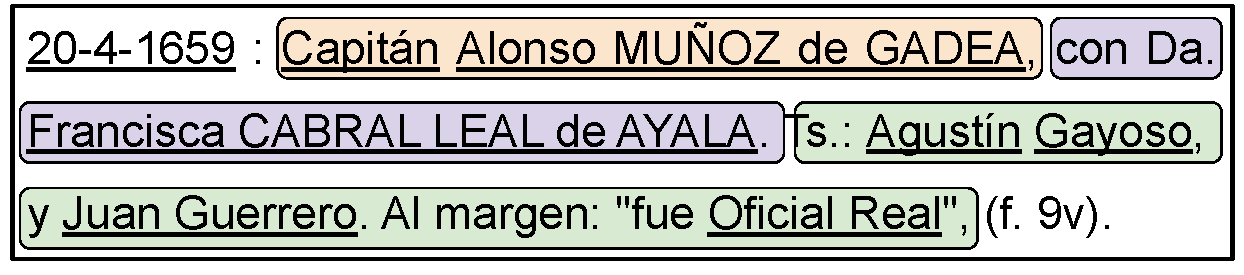
\includegraphics[width=\linewidth]{Figures/marriageDocumentnoParents.pdf}
    \caption{}
  \end{subfigure}
  \begin{subfigure}{.23\textwidth}
    \centering
    \bipartiteNoParents{1}
  \end{subfigure}
  \begin{subfigure}{.23\textwidth}
    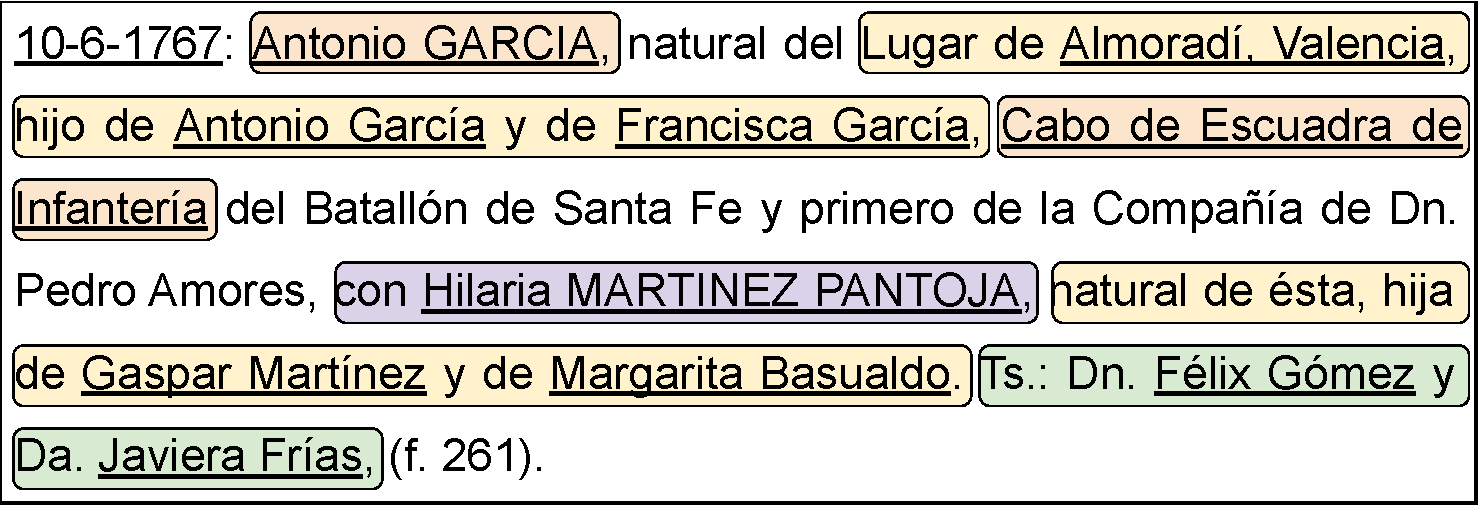
\includegraphics[width=\linewidth]{Figures/marriageDocument.pdf} 
    \caption{}
    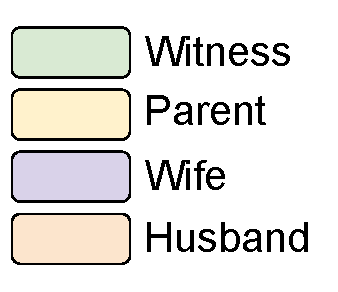
\includegraphics[scale=0.2,left]{Figures/MarriageLegend.pdf}
  \end{subfigure}
  \centering
  \begin{subfigure}{.23\textwidth}
    \bipartiteParents{1}
  \end{subfigure}
    
    
    % 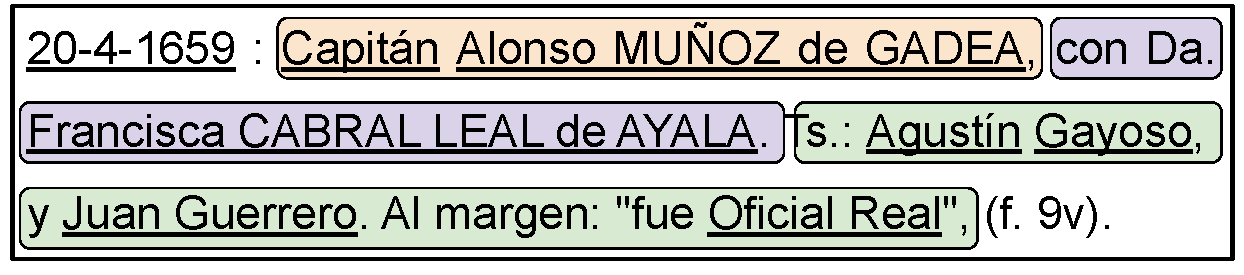
\includegraphics[width=0.49\linewidth]{Figures/marriageDocumentnoParents.pdf} 
    % \bipartiteNoParents{1}
    % % \subfigure[]{\bipartiteNoParents{0.6}} 

    % 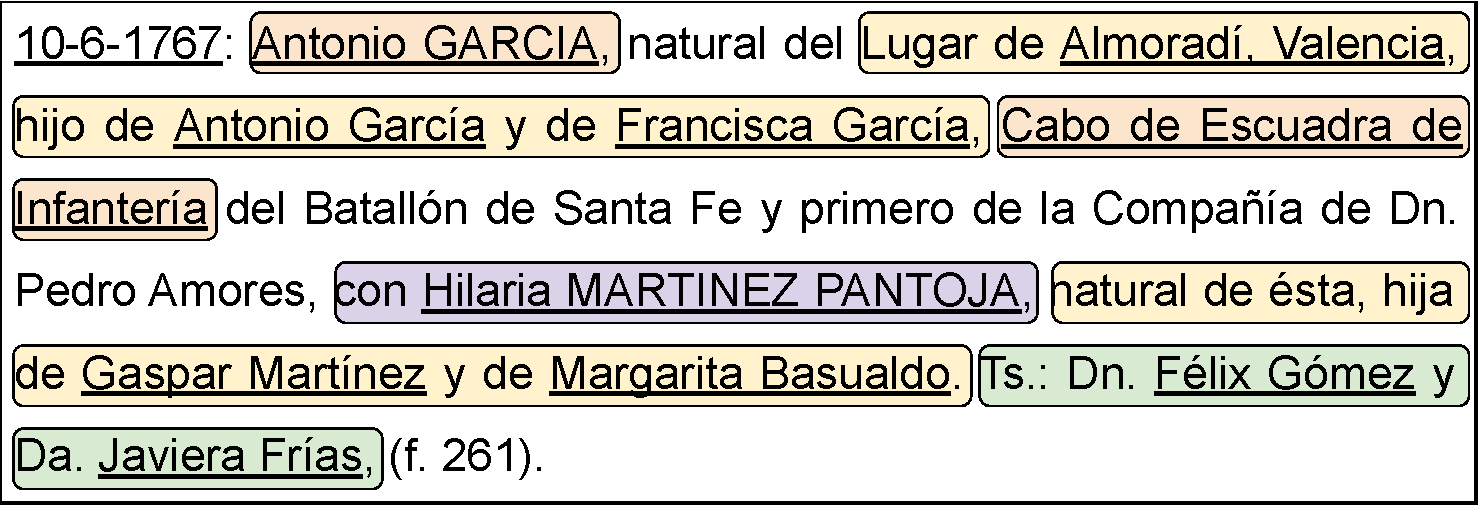
\includegraphics[width=0.49\linewidth]{Figures/marriageDocument.pdf}
    % \bipartiteParents{1}
    
    \caption{Transformation of annotated marriage acts from use case \zacarias\ into our proposed model. The acts can refers to parent relationships (b) or not (a). Each color represent a relationship between a person and an event. Additional information on the persons or the events are underlined and stored in the nodes as attributes. The network is a concrete representation of the events mentioned in the original sources. H: Husband, W: wife, T1,T2: witnesses, M: marriage act, HF, HM, WF, WM: husband/wife's father/mother.
    % \jdf{Tu peux expliquer les A, B, T1, T2, PA, MA, PB, MB?}
    }\label{tab:MarriageModel}
\end{figure}
\fi


% \definecolor{associate}{rgb}{1, 0, 1}
% \definecolor{guarantor}{rgb}{0, 0, 1.0}
% \definecolor{approbator}{rgb}{0, 1, 0}

\colorlet{associate}{orange!80!white!50}
\colorlet{guarantor}{blue!80!white!50}
\colorlet{approbator}{olive!80!white!50}

% \colorlet{approbator}{LimeGreen}

\newcommand{\simplePiemont}[1][0]{\begin{tikzpicture}[node distance=3cm, auto]
        \node[shape=circle,draw=gray, fill=lightgrey] (A1) at (2,1) {A1};
        \node[shape=circle,draw=gray, fill=lightgrey] (A2) at (2.75,3) {A2};
        \node[shape=circle,draw=gray, fill=lightgrey] (A3) at (3.5,1) {A3};
        \node[shape=circle,draw=gray, fill=lightgrey] (G) at (1.5,2.1) {G};
        \node[shape=circle,draw=gray, fill=lightgrey] (Ap) at (4,2.1) {Ap};
    
        \begin{scope}[every node/.style={scale=.5}]
            \path [line width=0.5mm]
            (A1) edge node [above left, color=black] {\small 1712} (A2)
            (A1) edge node [color=black] {\small 1712} (A3)
            (A2) edge node [color=black] {\small 1712} (A3)
            (G) edge node [right, color=black] {\small 1712} (A1)
            (G) edge node [right, color=black] {\small 1712} (A2) 
            (G) edge node [right, color=black] {\small 1712} (A3)
            (Ap) edge node [right, color=black] {\small 1712} (A1)
            (Ap) edge node [right, color=black] {\small 1712} (A2) 
            (Ap) edge node [right, color=black] {\small 1712} (A3)
            (G) edge node [color=black] {\small 1712} (Ap); 
        \end{scope}
    \end{tikzpicture}}

\newcommand{\unipartitePiemont}[1][0]{\begin{tikzpicture}[->, node distance=3cm, auto]
        \node[shape=circle,draw=gray, fill=lightgrey] (A1) at (2,1) {A1};
        \node[shape=circle,draw=gray, fill=lightgrey] (A2) at (2.75,3) {A2};
        \node[shape=circle,draw=gray, fill=lightgrey] (A3) at (3.5,1) {A3};
        \node[shape=circle,draw=gray, fill=lightgrey] (G) at (1.5,2.1) {G};
        \node[shape=circle,draw=gray, fill=lightgrey] (Ap) at (4,2.1) {Ap};
    
        \begin{scope}[every node/.style={scale=.5}]
            \path [line width=0.5mm]
            (A1) edge [color=associate] node [above left, color=black] {\small 1712} (A2)
            (A1) edge [color=associate] node [color=black] {\small 1712} (A3)
            (A2) edge [color=associate] node [color=black] {\small 1712} (A3)
            (G) edge [color=guarantor] node [right, color=black] {\small 1712} (A1)
            (G) edge [color=guarantor] node [right, color=black] {\small 1712} (A2) 
            (G) edge [color=guarantor] node [right, color=black] {\small 1712} (A3)
            (Ap) edge [color=approbator] node [right, color=black] {\small 1712} (A1)
            (Ap) edge [color=approbator] node [right, color=black] {\small 1712} (A2) 
            (Ap) edge [color=approbator] node [right, color=black] {\small 1712} (A3); 
        \end{scope}
    \end{tikzpicture}}
    
    
\newcommand{\bipartitePiemont}[1][0]{\begin{tikzpicture}[, node distance=3cm, auto]
        \node[shape=circle,draw=gray, fill=lightgrey] (A1) at (0,3) {A1};
        \node[shape=circle,draw=gray, fill=lightgrey] (A2) at (0,2) {A2};
        \node[shape=circle,draw=gray, fill=lightgrey] (A3) at (0,1) {A3};
        
        \node[shape=circle,draw=gray, fill=lightgrey] (G) at (3,3) {G};
        \node[shape=circle,draw=gray, fill=lightgrey] (Ap) at (3,1) {Ap};
        
        \node[shape=rectangle,draw=gray, align=center,fill=lightgrey] (D) at (1.5,2) {M \\[0.5em] \small 1761};
        \draw (D.west) -- (D.east);
    
        \begin{scope}[every node/.style={scale=.5}]
            \path [line width=0.5mm] (A1) edge [color=associate] (D)
            (A2) edge [color=associate] (D)
            (A3) edge [color=associate] (D)
            (G) edge [color=guarantor] (D)
            (Ap) edge [color=approbator] (D);
        \end{scope}
        \end{tikzpicture}}
        
        

% \definecolor{father}{rgb}{1, 0, 1}
\colorlet{father}{red!80!white!50}
\colorlet{mother}{green!80!white!50}
\colorlet{child}{blue!80!white!50}

% \definecolor{mother}{rgb}{0, 0, 1.0}
% \definecolor{child}{rgb}{0, 1, 0}


\newcommand{\birthSimple}[1][0]{\begin{tikzpicture}[, node distance=3cm, auto]
        \node[shape=circle,draw=gray, fill=lightgrey] (F) at (0,1) {F};
        \node[shape=circle,draw=gray, fill=lightgrey] (M) at (1.5,1) {M};
        \node[shape=circle,draw=gray, fill=lightgrey] (C) at (0.75,0) {C};
    
        \begin{scope}[every node/.style={scale=.5}]
            \path [line width=0.5mm] (F) edge [color=black] node [above right, color=black] {\small 1901} (C)
            (M) edge node [above left, color=black] {\small 1901} (C)
            (F) edge node [color=black] {\small 1901} (M);
        \end{scope}
        \end{tikzpicture}}

\newcommand{\birthUnipartite}[1][0]{\begin{tikzpicture}[, node distance=3cm, auto]
        \node[shape=circle,draw=gray, fill=lightgrey] (F) at (0,1) {F};
        \node[shape=circle,draw=gray, fill=lightgrey] (M) at (1.5,1) {M};
        \node[shape=circle,draw=gray, fill=lightgrey] (C) at (0.75,0) {C};
    
        \begin{scope}[every node/.style={scale=.5}]
            \path [line width=0.5mm] (F) edge [color=father] node [above right, color=black] {\small 1901} (C)
            (M) edge [color=mother] node [above left, color=black] {\small 1901} (C);
        \end{scope}
        \end{tikzpicture}}
        
\newcommand{\birthBipartite}[1][0]{\begin{tikzpicture}[, node distance=3cm, auto]
        \node[shape=circle,draw=gray, fill=lightgrey] (F) at (0,2) {F};
        \node[shape=circle,draw=gray, fill=lightgrey] (M) at (2,2) {M};
        \node[shape=rectangle,draw=gray, align=center,fill=lightgrey] (D) at (1,1) {M \\[0.5em] \small 1901};
        \draw (D.west) -- (D.east);
        \node[shape=circle,draw=gray, fill=lightgrey] (C) at (1,0) {C};
    
        \begin{scope}[every node/.style={scale=.5}]
            \path [line width=0.5mm] (F) edge [color=father] (D)
            (M) edge [color=mother] (D)
            (D) edge [color=child] (C);
        \end{scope}
        \end{tikzpicture}}
        
        
    %      \hline Original Document & Co-occurrence & Unipartite representation & Proposed model \\
    % \hline \centering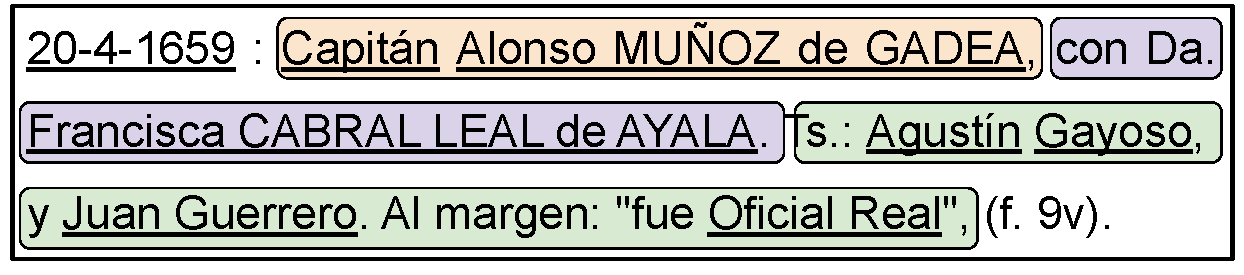
\includegraphics[scale=0.3]{Figures/marriageDocumentnoParents} & \simple & \centering\noParents & \bipartiteNoParents \\
    % \hline doc & \simplePiemont & \centering\unipartitePiemont & \bipartitePiemont \\
    % \hline doc & \birthSimple
% % Table with unipartite graphs
\begin{table*}
    % \begin{tabular}{ | m{20em} | m{15em} | m{20em} | }
    \begin{tabular}{|m{6cm}|m{3cm}|m{3cm}|m{4cm}|}
    \hline Original Document & Co-occurrence & Unipartite representation & Bipartite \\
    \hline
    % \centering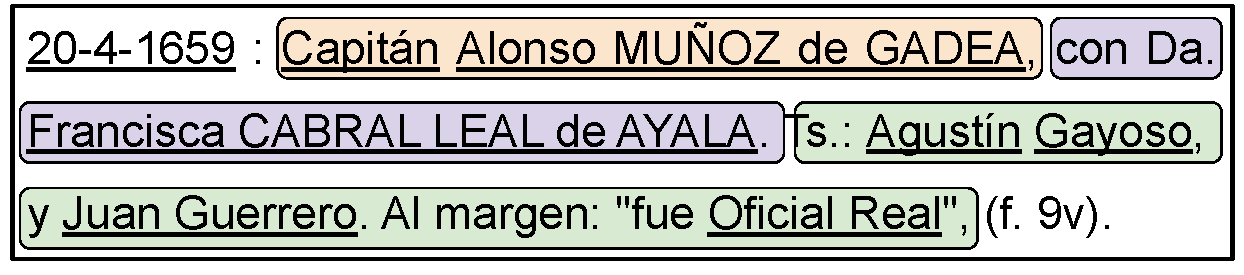
\includegraphics[scale=0.3]{Figures/marriageDocumentnoParents}
    20-4-1659 : \colorbox{epoux}{Capitán Alonso MUÑOZ de GADEA}, con Da. \colorbox{epouse}{Francisca CABRAL LEAL de AYALA}. Ts.: \colorbox{temoin}{Agustín Gayoso}, y \colorbox{temoin}{Juan Guerrero. Al margen: "fue Oficial Real"}, (f. 9v). \linebreak
    \colorbox{epoux}{Husband} \colorbox{epouse}{Wife} \colorbox{temoin}{Witness}
    & \centering\simple & \centering\noParents & \bipartiteNoParents \\
    \hline 1712: Construction of a church in Torino. 
    Associates: \colorbox{associate}{Bellotto G, Bello P.M, Bello G.}
    Guarantor: \colorbox{guarantor}{ Astrano G.A.}
    Approbator: \colorbox{approbator}{Corte A.} \linebreak
    \colorbox{associate}{Associate} \colorbox{guarantor}{Guarantor} \colorbox{approbator}{Approbator}
    & \centering\simplePiemont & \centering\unipartitePiemont & \bipartitePiemont \\
    \hline Le 7 octobre 1901, \colorbox{father}{François Marie Esnault} et \colorbox{mother}{Marie Julie Léopoldine Colson} ont déclaré la naissance de leur fille, nommée \colorbox{child}{Blanche Esnault} dans la commune de Saint-Maur-des-Fossés.
    \linebreak
    \colorbox{father}{Father} \colorbox{mother}{Mother} \colorbox{child}{Child}
    & \centering\birthSimple & \centering\birthUnipartite & \birthBipartite\\
    \hline
    
    % & \begin{center}\bipartiteNoParents\end{center} \\
    
        % \hline Original Document & Unipartite representation & Proposed model \\
        % \hline \centering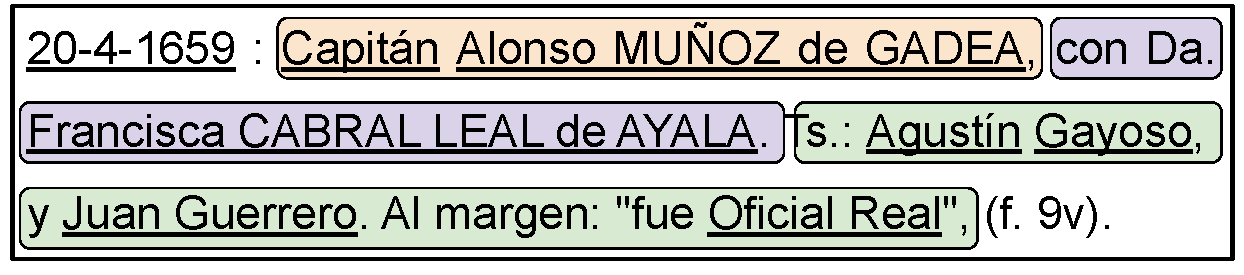
\includegraphics[scale=0.3]{Figures/marriageDocumentnoParents}\\
        % 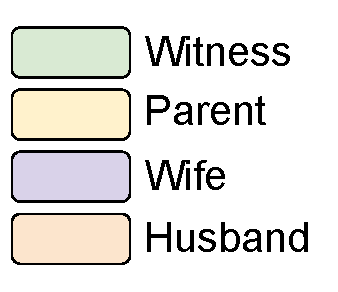
\includegraphics[scale=0.2,right]{Figures/MarriageLegend.pdf} & \begin{center}\noParents\end{center} & \begin{center}\bipartiteNoParents\end{center} \\
        % \hline 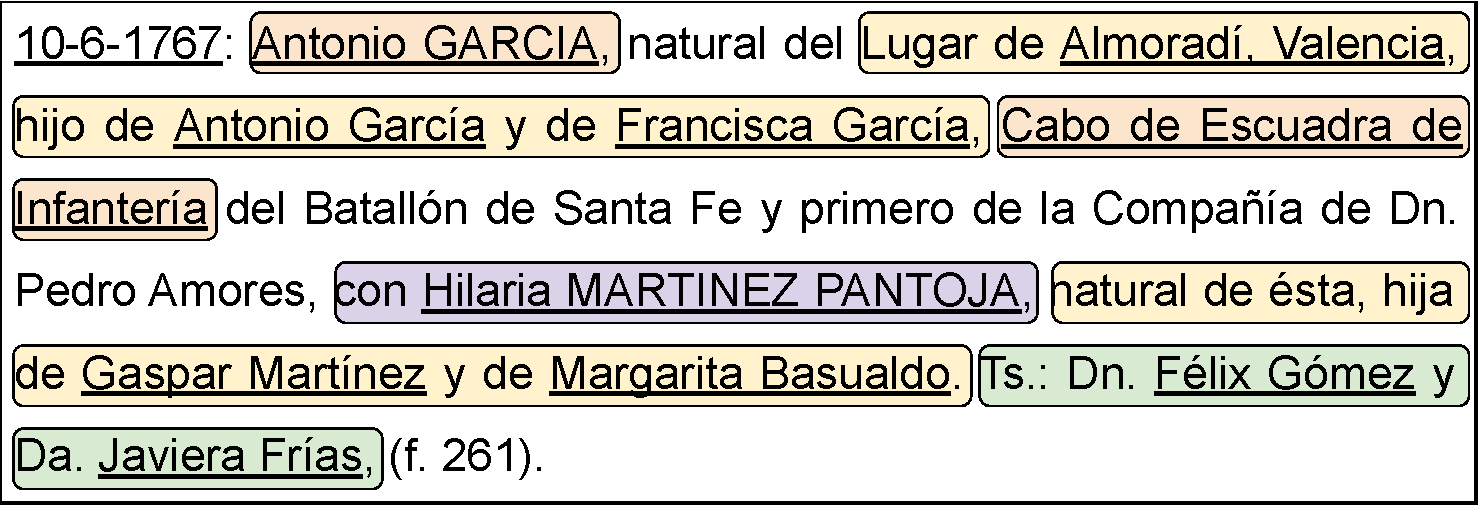
\includegraphics[scale=0.25]{Figures/marriageDocument} & \unipartiteParents & \bipartiteParents \\
        % \hline
    \end{tabular}
    \caption{Resulting networks using different models produced by one document of the examples detailed in \autoref{sec:examples}: co-occurrence, unipartite and bipartite models.   }\label{tab:models}
\end{table*}

\subsection{Bipartite Multivariate Dynamic Social Network}

We argue that most historical sources are well modeled by bipartite networks when doing an HSNA. Moreover, recent studies try to incorporate attribute information, particularly the time and location, but also potentially other quantitative information.
We therefore propose a document-oriented data model for social networks, grounded on historical sources and persons, unifying the models of PUCK and Jigsaw, with the following properties:
\begin{description}[noitemsep]
\item[{Bipartite:}] There are two types of nodes, persons and events or documents. An event, such as a marriage, is most of the time witnessed by a document, but we refer to them interchangeably as events and documents. A link models the reference of a person in a document. In a social network, events can be of the same sub-type, such as contracts, or of multiple sub-types, e.g., for genealogy: \emph{birth certificates}, \emph{death certificates}, \emph{marriage acts}.
\item[Roles:] Links have a type corresponding to the \emph{roles} of the persons in the event. For a marriage act, the roles include \emph{wife}, \emph{husband}, \emph{witness}. This is a key aspect of our model since it clarifies the relationship between the persons within a event.
\item[{Multivariate:}] The nodes can have attributes, which give additional information on the persons and events. Persons nodes usually have information on their sex or profession. Events have a date, sometimes a location, and potentially other information such as their sub-type.
\item[{Geolocated:}] Events should have a location with a given longitude and latitude. 
\item[{Dynamic:}] Events are always dated. We rely on this date since it encodes the social dynamics of the network.
\end{description}

From the examples of \autoref{tab:models}, we leverage 3 properties of this model:
\begin{enumerate}[noitemsep]
    \item \textbf{No information loss:} When projecting the original source into a person-to-person network, we cannot trace the original events links refer to. We know if pairs of persons have been in events together, but it become impossible to know which one. Moreover, we lose the fact that more than two persons appear in the same event together, as relationships become pairwise only.   
    \item \textbf{No duplication:} When using document nodes, the information related to the events such as the time and location can be directly tied to those node, whereas the same information is duplicated in several links when projecting the data into an unipartite network.
    \item \textbf{No distorsion:} Most relationships referred in documents are complex and are complicated to model as pairwise relations. Creating a unipartite network often create some bias as several coexistant representation may coexist. In contrary, bipartite network represent well the reality of the social relationships, as they model the data as it is written in the documents.
\end{enumerate}


\section{Applications}

After constructing their network, historians can explore and analyze them using specifically designed visual analytics tools. 
We designed ComBiNet \cite{pister2022visual} to explore this type of historic dataset modeled as bipartite multivariate dynamic networks and to help social scientists answer their questions with the help of visual queries and interactive comparisons. \autoref{fig:combinet} shows the interface to compare two meaningful groups in example \pascal. We can see that exploring the historic dataset modeled as \modelplural allow to answer complicated questions related to the constructions themselves instead of only the persons. In this example, we can see the \textit{Zo} family have more construction contracts in \textit{Turin Territoire} than the \textit{Menafoglio} family.

\begin{figure}[tb]
 \centering % avoid the use of \begin{center}...\end{center} and use \centering instead (more compact)
 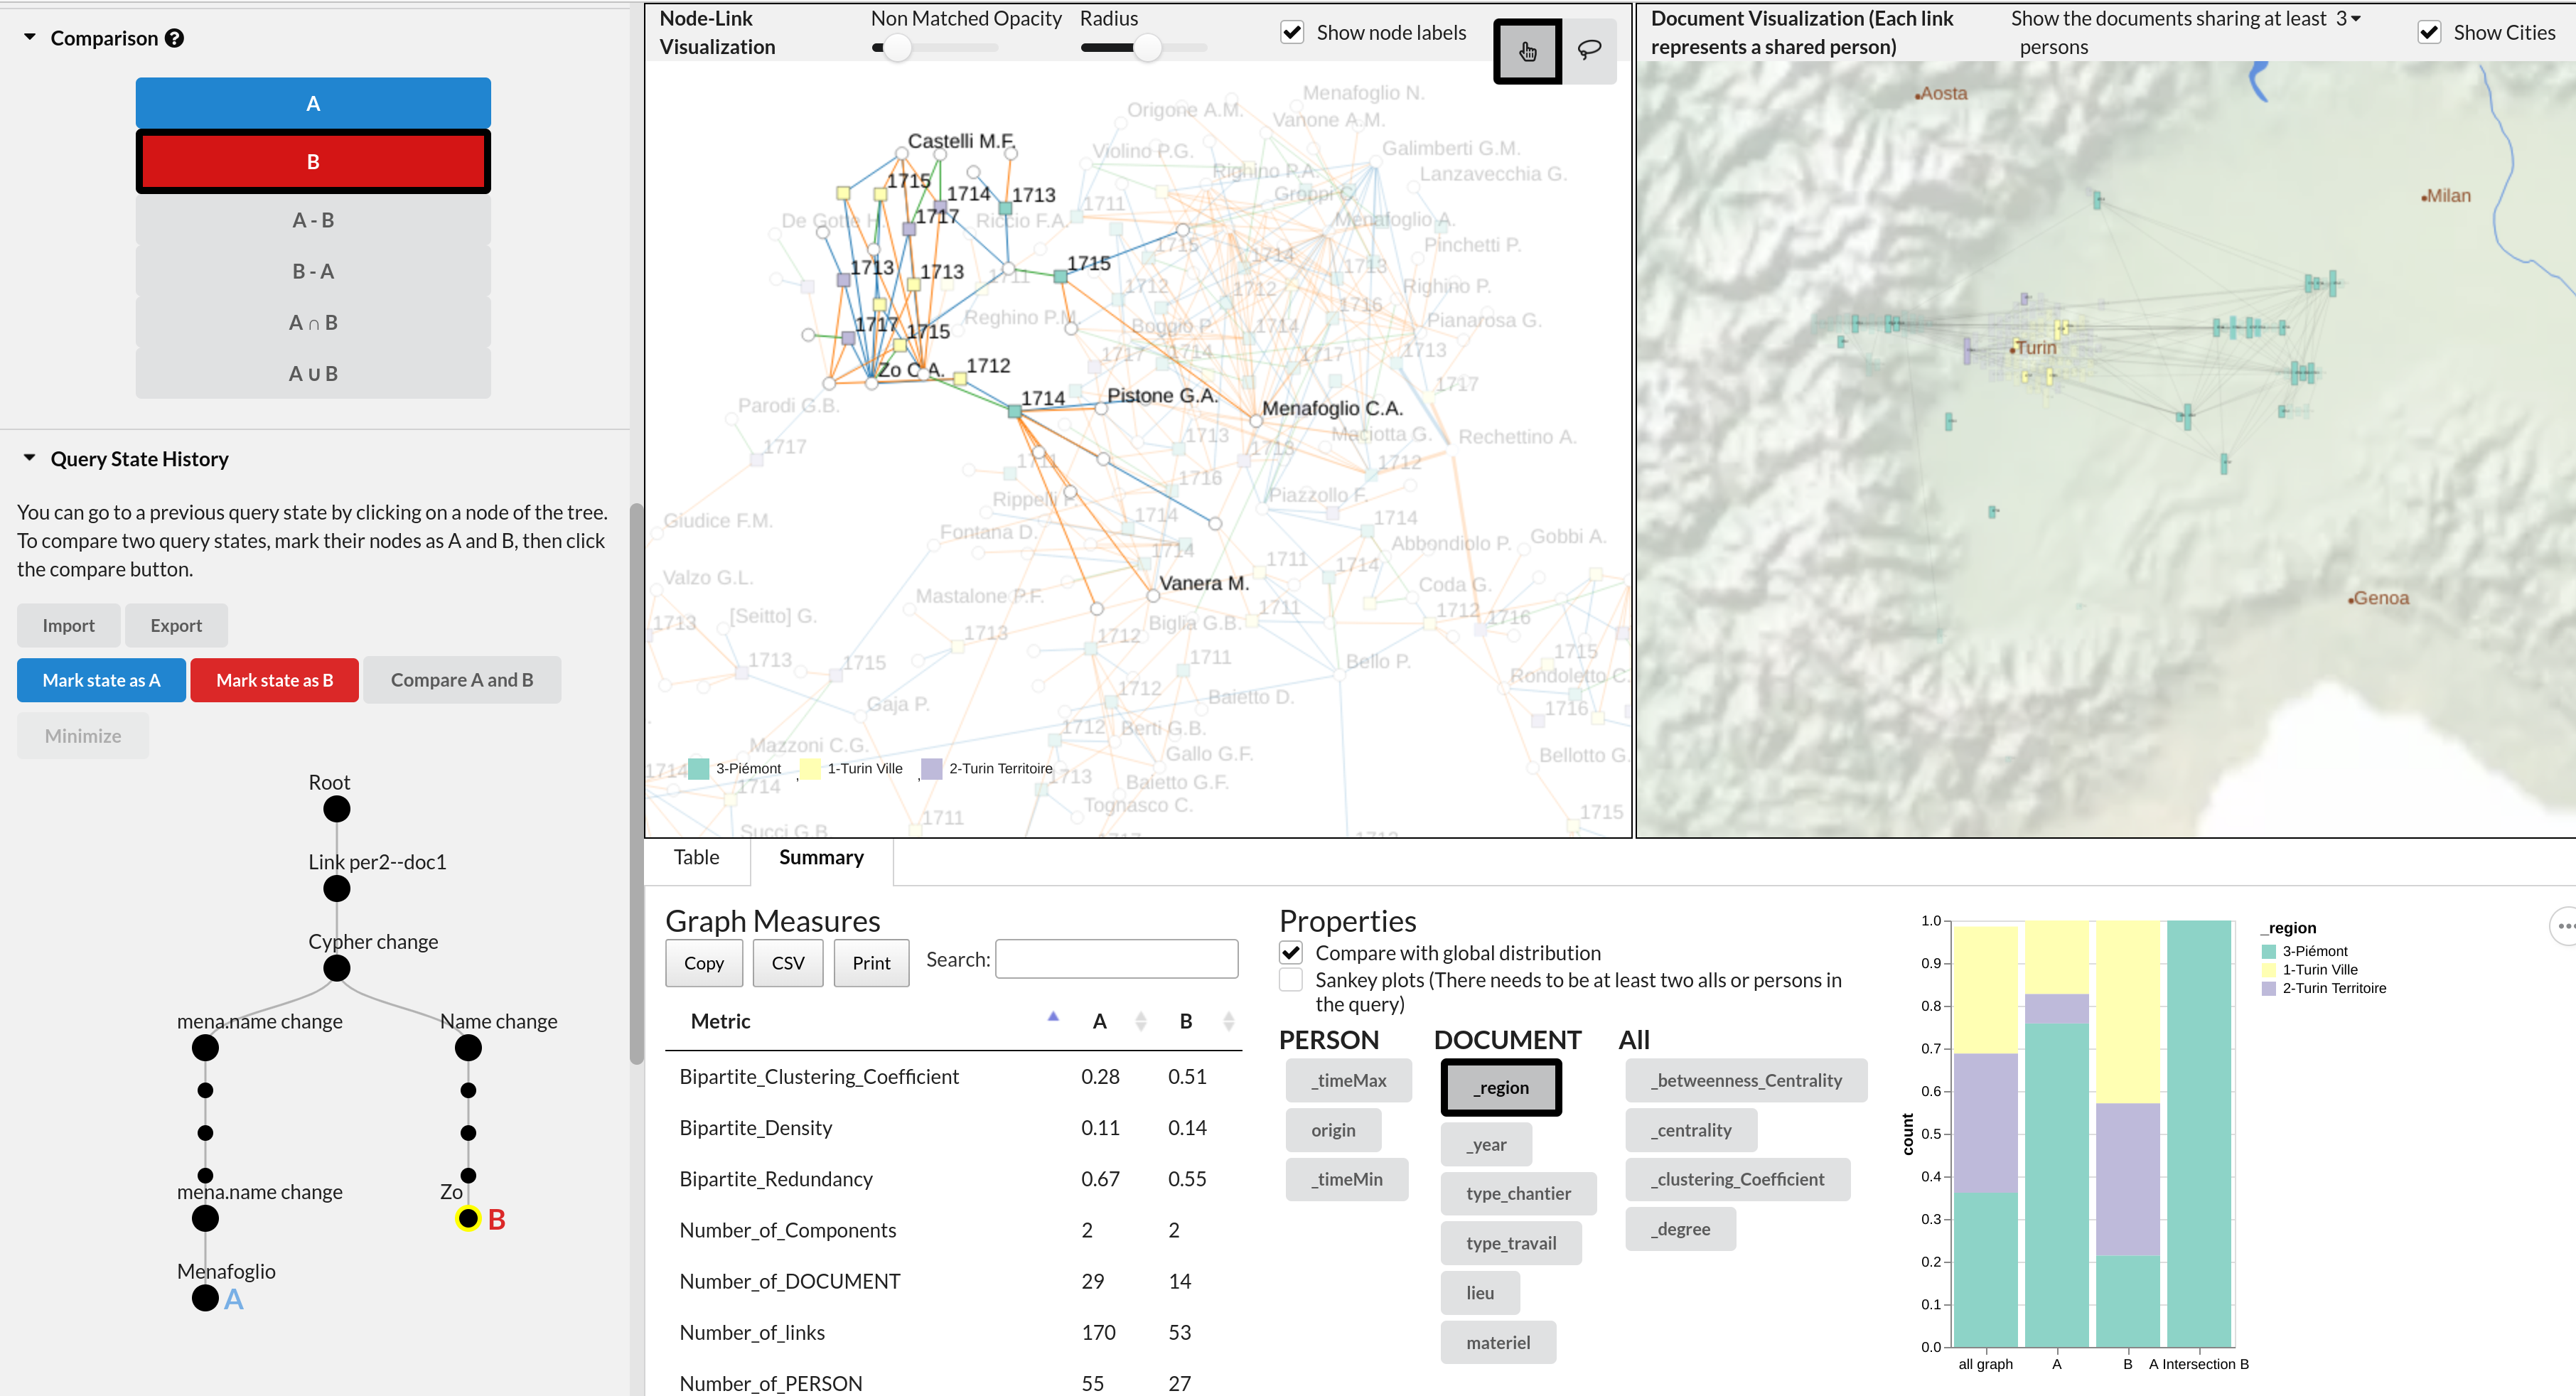
\includegraphics[width=\columnwidth]{Figures/ComBiNet.png}
 \caption{ComBiNet interface exploring example \pascal. The left menu let users filter the data and compare groups. The center view shows the bipartite network with a node-link diagram. The right view show a map with the geolocated construction contracts. The bottom view give measures and attribute distributions related to the network and the current filters and comparisons. 
 The user currently compare the \textit{Menafoglio} and \textit{Zo} families in terms of their construction types and close relationships.}
 \label{fig:combinet}
\end{figure}


\section{Discussion}

We propose a way of modeling the majority of historical document datasets using \modelplural, as it satisfy \textit{reality} and \textit{traceability} properties in relation to the original documents. 
We also argue for the elaboration of visual analytics tools to explore and analyze this type of data. However, other network models could be better suited for answering some questions or to represent specific underlying phenomena. Simple network models such as co-occurrence networks can be effective to answer simple questions related to the centrality for example, while more complex models such as multipartite networks could also be used to model more complex entities.
However, we think using \modelplural as a first step in the analysis is a good way of stepping in the network domain space while keeping the traceability to the original sources, and can be used easily to create other networks with the help of projections and transformations \cite{andrei2011porgy}. 


\section{Conclusion}

HSNA is a complicated process which starts from the collection of historical documents and ends with the elaboration of high level sociological conclusions supported by the analysis of a network modeling the social relationships of individuals, extracted from the documents. 
Most HSNA studies focus on studying the network they have constructed to leverage insights, and give less details on the annotation and network construction process. It can therefore be hard for readers to link the network shape and analysis results back to the original sources and do not allow any replicability of the analysis. Furthermore, historical sources are often complex, and using a wrong or too simple network model can bias the final analysis.
We argue in favor of modeling historical sources as \modelplural as it allows to model the documents as they are and allowing an easy traceability from the network space to the original documents.
Moreover, with the help of real examples, we show that this model enforce no information loss, no duplication and no distortion compared to other network models. It therefore allows to model all the complexity of historical documents into a network, that historians can visualize and analyze with specific tools to make sociological conclusions.



%% if specified like this the section will be committed in review mode
\acknowledgments{
The authors wish to thank A, B, and C. This work was supported in part by
a grant from XYZ.}

%\bibliographystyle{abbrv}
\bibliographystyle{abbrv-doi}
%\bibliographystyle{abbrv-doi-narrow}
%\bibliographystyle{abbrv-doi-hyperref}
%\bibliographystyle{abbrv-doi-hyperref-narrow}

\bibliography{main}
\end{document}
